\documentclass[11pt]{article}
\usepackage{subfigure,wrapfig,booktabs,fancyhdr,amsmath,amsfonts,float}
\usepackage[pdftex]{graphicx}
\usepackage{bm,amssymb,amsmath,amsthm,wasysym,color,fullpage,setspace,multirow}
\usepackage{listings}
\lstset{language=Matlab}

\newcommand{\vb}{\boldsymbol}
\newcommand{\vbh}[1]{\hat{\boldsymbol{#1}}}
\newcommand{\vbb}[1]{\bar{\boldsymbol{#1}}}
\newcommand{\vbt}[1]{\tilde{\boldsymbol{#1}}}
\newcommand{\vbs}[1]{{\boldsymbol{#1}}^*}
\newcommand{\vbd}[1]{\dot{{\boldsymbol{#1}}}}
\newcommand{\vbdd}[1]{\ddot{{\boldsymbol{#1}}}}
\newcommand{\by}{\times}
\newcommand{\tr}{{\rm tr}}
\newcommand{\cpe}[1]{\left[{#1} \times \right]}
\newcommand{\sfrac}[2]{\textstyle \frac{#1}{#2}}
\newcommand{\ba}{\begin{array}}
\newcommand{\ea}{\end{array}}
\renewcommand{\earth}{\oplus}
\newcommand{\sinc}{{\rm \hspace{0.5mm} sinc}}
\newcommand{\tf}{\tilde{f}}
\newcommand{\tbox}[1]{\noindent \fbox{\parbox{\textwidth}{#1}}}
\DeclareMathAlphabet{\mathpzc}{OT1}{pzc}{m}{it}

% Weird thing I have to add to allow `rubber` to compile
\DeclareUnicodeCharacter{2212}{-}

\title{ASE 389P-7 \\ Exam 1}
\author{Alejandro Moreno}\date{October 4, 2022}

\begin{document}
%\onehalfspace
\maketitle

\section{Problem 1}

\subsection{Instruction}

Write a function in Matlab that simulates the train-horn-Doppler scenario
discussed in lecture. Assume that the train tracks are rectilinear.

Be sure to account for the nonzero time of flight $\delta t_{TOF}$ as discussed
in lecture. The effect of $\delta t_{TOF} > 0$ is that the stationary observer
will discern an $f_D$ at time $t_k$ that relates to the train’s line-of-sight
velocity at time $t_k − \delta t_{TOF}$. More precisely, the apparent frequency
of the train horn at the location of the observer at time $t_k$ is given by

\begin{equation}
	f_r(t_k) = \frac{f_c}{1 + \frac{v_{los}(t_k)}{v_s}}
\end{equation}

where $f_c$ is the nominal horn frequency, $v_{los}(t_k)$ is the line-of-sight
velocity at $t_k$, and $v_s$ is the speed of the signal in the medium. Note that
the line-of-sight geometry used to calculate $v_{los}(t_k)$  is between the
observer at time $t_k$ and the horn at time $t_k − \delta t_{TOF}$.

Download the audio file trainout.wav from Canvas. This file was created with the
following input argument values:

\begin{lstlisting}
  fh = 440;
  vTrain = 20;
  t0 = 0;
  x0 = 0;
  delt = 0.01;
  N = 1000;
  vs = 343;
\end{lstlisting}

Set up your simulator with these same values. Estimate the values of xObs and
dObs by adjusting them in your simulation until you get an apparent received
frequency profile that matches the one in the audio file.

\subsection{MATLAB code}

\lstinputlisting{simulateTrainDoppler.m}
\lstinputlisting{topSimulateTrainDoppler_temp.m}

\subsection{Result}

Analizing the given signal it's possible to manually tag the moment in which the
train passed in front of the receiver. Figure~\ref{fig:spectrogram_original}
shows how the power density is concentrated at higher frequency before 3.069 sec
and drops rapidly after that. This indicates the exact moment at which the train
passed infront of the receiver.

\begin{figure}[H]
	\centering
	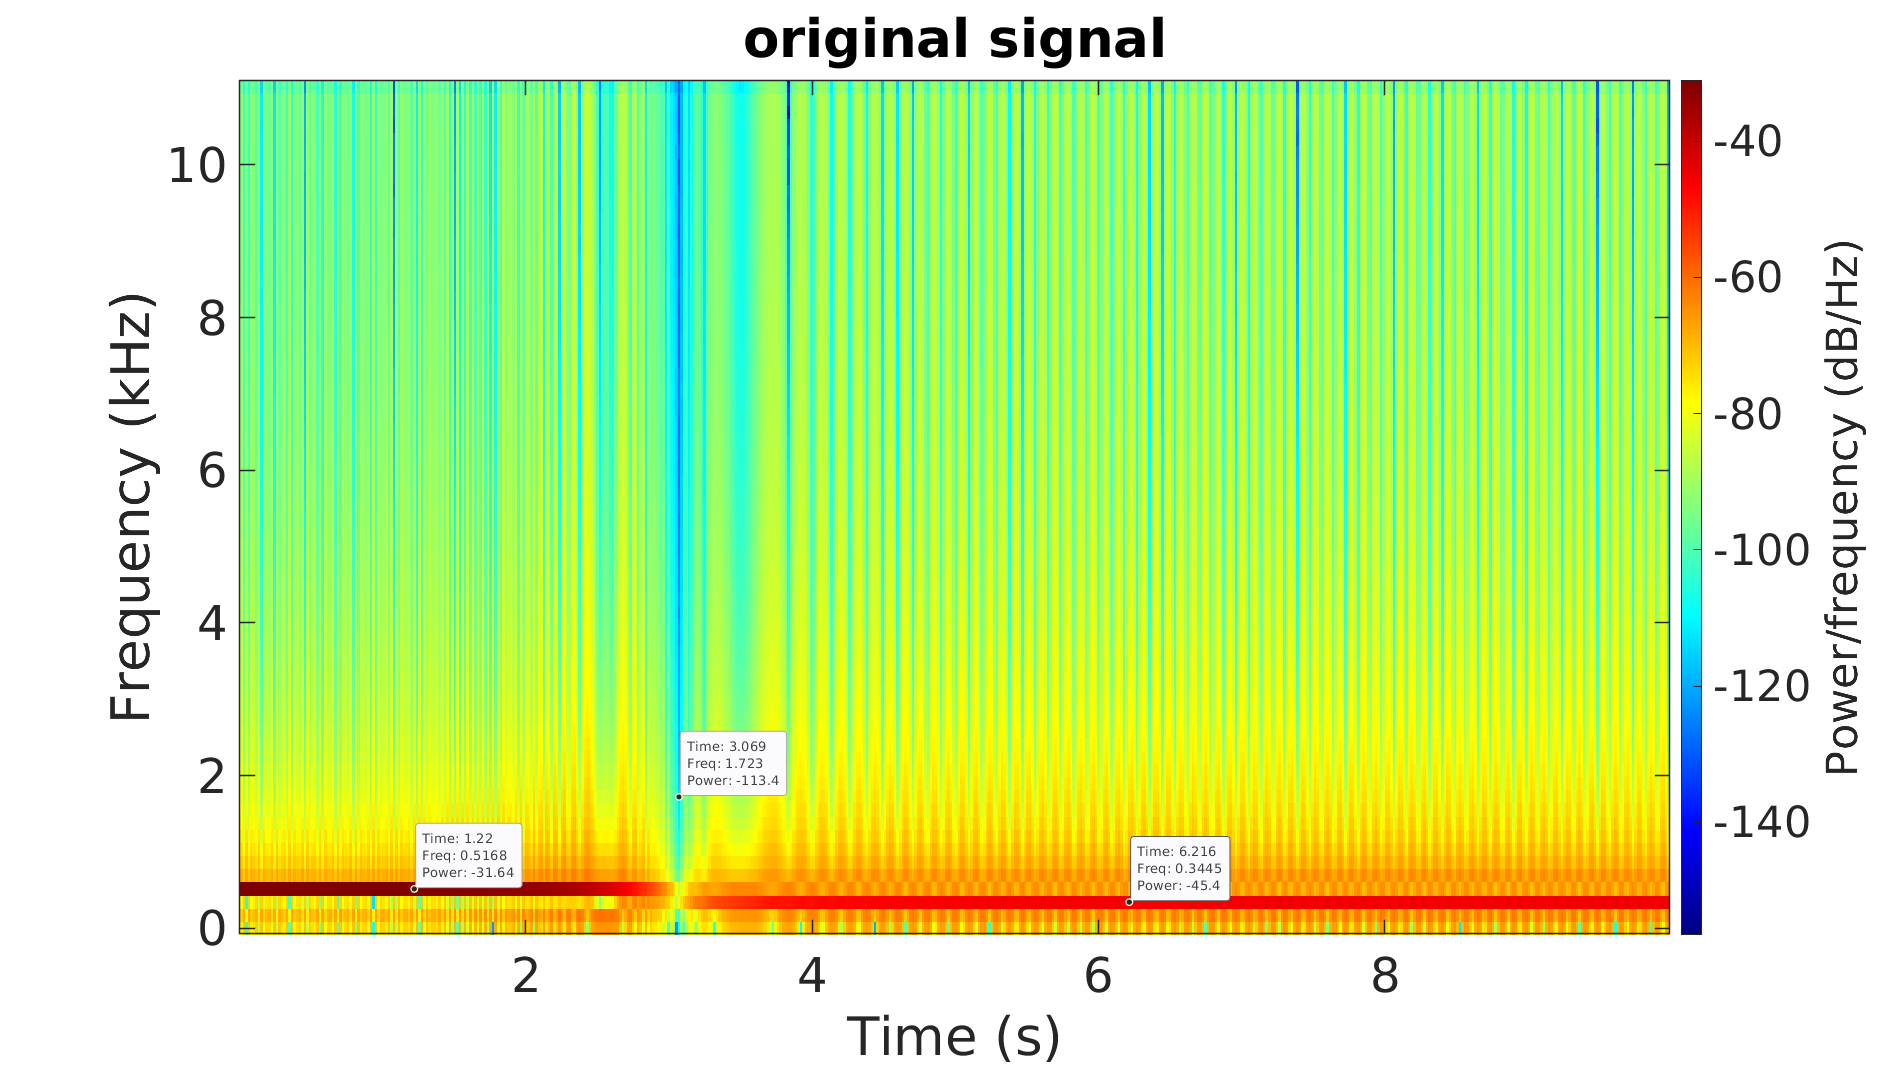
\includegraphics[width=0.9\textwidth]{figs/ex1_spectrogram_orig.png}
	\caption{Spectrogram of the given signal.}
	\label{fig:spectrogram_original}
\end{figure}

This, approach lead to $xObs = 56.8$ and $dObs = 10$.




\section{Problem 2}

\subsection{Instruction}

Show that the group velocity vg and the phase index of refraction np are related
by $v_g = c \eta_p$ for small group and phase velocity departures from the speed
of light $c$.

\subsection{Solution}



\section{Problem 3}

\subsection{Instruction}

In lecture we considered an analog signal $x_a (t)$ sampled by impulses:

\begin{equation}
	x_\delta (t) = \sum_{n=-\infty}^{\infty} x_a(nT) \delta(t-nT)
	\label{eq:ex3_analog_signal}
\end{equation}

We showed that the Fourier transform of the impulse-sampled signal $x_\delta (t)$
is related to $X_a (f)$, the Fourier transform of $x_a (t)$, by

\begin{equation}
	X_\delta (f) = \frac{1}{T} \sum_{n=-\infty}^{\infty} X_a(f- \frac{n}{T})
	\label{eq:ex3_FT_sampled_signal}
\end{equation}

We can derive a similar relationship between $X_a (f)$ and the Fourier transform
of the discrete-time signal

\begin{equation}
	x(n) = x_a (nT), − \infty < n < \infty
\end{equation}

To make this easier, we’ll define the frequency variable
$\tilde{f} = f T = \frac{f}{f_s}$. This variable, which has units of cycles per
sample and is often called the normalized frequency, is used as the frequency
variable for discrete-time signals. For example, a discrete-time sinusoid can be
represented as $2x(n) = cos(2\pi \tilde{f}n)$. For discrete-time signals, only
frequencies in the range $− 1/2 \le \tilde{f} \le 1/2$ are unique;
all frequencies $|\tilde{f}| > 1/2$ are aliases.

The Fourier transform of a discrete-time signal $x(n)$ is defined by

\begin{equation}
	X(\tilde{f}) = \sum_{n=-\infty}^{\infty} x(n) \exp{(-j 2 \pi \tilde{f} n)}
	\label{eq:ex3_DFT}
\end{equation}

and the inverse transform is defined by

\begin{equation}
	x(n) = \int_{-1/2}^{1/2} X(\tilde{f}) \exp{(j 2 \pi \tilde{f} n)} d\tilde{f}
	\label{eq:ex3_IDFT}
\end{equation}

Derive the relationship between $X(\tilde{f})$ and $X_a (f)$.

\textbf{Hint:} This is a standard relationship whose derivation can be found in
many texts that treat digital signal processing. You’re free to use such a text
as a guide or you may perform the derivation yourself following these steps:

\begin{itemize}
	\item Express $x(n) = x_a (nT)$ in terms of $X_a (f)$.
	\item Equate this expression with the inverse transform definition given above.
	\item Express the integral that goes from $−\infty to \infty$ as an infinite
	      sum of integrals of width $f_s$.
	\item Make a change of variable $f = \tilde{f}  fs$ in this infinite sum of
	      integrals expression to eliminate $f$ in favor of $\tilde{f}$.
	\item Make some deductions to arrive at the desired relationship between
	      $X(\tilde{f})$ and $X_a (f = \tilde{f}·fs )$.
\end{itemize}

\subsection{Solution}

It is possible to consider equation~\ref{eq:ex3_analog_signal} to calculate the
Fourier Transform of $x_\delta(t)$.

\begin{equation}
	X_\delta (f) = \frac{1}{T} \sum_{n=-\infty}^{\infty} X_a(f- \frac{n}{T})
	= \sum_{n=-\infty}^{\infty} x_a(nT) \exp{(-j 2 \pi f n T)}
\end{equation}

Then, it is possible to see that formula for $X_\delta (f)$ can be equated to
\ref{eq:ex3_DFT} as follows

\begin{equation}
	X_\delta (f) = \sum_{n=-\infty}^{\infty} x_a(nT) \exp{(-j 2 \pi f n T)}
	= \sum_{n=-\infty}^{\infty} x(n) \exp{(-j 2 \pi \tilde{f} n)}
	= X(\tilde{f})
\end{equation}

This leads to the following relationship

\begin{equation}
	X(\tilde{f}) = X_\delta (\frac{\tilde{f}}{T})
\end{equation}

Now, using equation~\ref{eq:ex3_FT_sampled_signal} it is possible to reach

\begin{equation}
	X(\tilde{f}) = \frac{1}{T} \sum_{n=-\infty}^{\infty} X_a(\frac{\tilde{f}- n}{T})
\end{equation}

\section{Problem 4}

\subsection{Instruction}

To measure the receiver temperature $T_R$ of a GNSS receiver and antenna setup,
a friend recommends placing the receiver’s antenna in a RF test enclosure such
as the one in the Radionavigation Laboratory (seen here
https://ramseytest.com/forensic-test-enclosures),
but cryogenically cooled down to 5 K, and then measuring the noise power in the
raw samples generated by the receiver. The enclosure effectively isolates the
antenna from environmental noise. The antenna is an active antenna consisting of
a patch element, a (passive) filter, and an amplifier. Is this a valid approach
for measuring TR ? Why or why not?

\subsection{Result}

The cryogenically cooled enclosure would only allow us to reduce the noise of
the receiver but not $T_A$. Therefore one could measure the noise power with and
without the cryogenically cooled enclosure and get an estimate of the $T_R$ by
substracting the results.

It seems like this is not a good idea though because if one would like to make the
best use of their money for the general usage of the GNSS receiver. Then, buying
the cryogenically cooled enclosure would only buy you a couple dBs better noise
performance. The main source of noise (the other GNSS signals one is not
interested in when aquiring from a particular satellite) would not be attenuated.
Therefore, one could measure the desired magnitude but that's it. No noticible
benefit would come from this purchase.



\section{Problem 5}

\subsection{Instruction}

Write a function in Matlab for computing the ionospheric delay from a model of
the ionosphere. Your function should adhere to the interface described on the
next page (which you can copy and paste as comments to your function). Only
develop calculations for the broadcast (Klobuchar) model. The function can later
be augmented to accommodate other model types. You can learn about the broadcast
model on pages 168-169 of the Misra and Enge text. More details can be found on
pages 128-130 of the GPS interface specification (IS) IS-GPS-200F.pdf posted on
Canvas. You will also need to write your own function for computing satellite
elevation and azimuth angles. Assume the WGS84 model for the shape of the Earth.
Note that the GPS IS uses semicircles as its angular measure, which is a strange
convention employed back in the 1970s to reduce memory and computation
requirement. The sin and cos functions in the IS (e.g., in Fig. 20-4) are meant
to operate on semicircles, unless otherwise indicated. Thus, when the IS writes,
e.g., $cos(\lambda_i −1.1617)$, where $\lambda_i$ is given in semicircles, you
can implement this in Matlab as $cos((\lambda_i −1.1617)\pi)$.

\subsection{Solution}


\begin{lstlisting}
function [delTauG] = getIonoDelay(ionodata,fc,rRx,rSv,tGPS,model)
% getIonoDelay : Return a model-based estimate of the ionospheric delay
%                experienced by a trans-ionospheric GNSS signal as it
%                propagates from a GNSS SV to the antenna of a terrestrial
%                GNSS receiver.
%
% INPUTS
%
% ionodata ------- Structure containing a parameterization of the
%                  ionosphere that is valid at time tGPS. The structure is
%                  defined differently depending on what ionospheric model
%                  is selected:
%
%                  broadcast --- For the broadcast (Klobuchar) model, ionodata
%                                is a structure containing the following fields:
%
%                       alpha0 ... alpha3 -- power series expansion coefficients
%                                            for amplitude of ionospheric delay
%                       beta0 ... beta3 -- power series expansion coefficients
%                                          for period of ionospheric plasma density 
%                                          cycle
%
%
% Other models TBD ...
%
% fc ------------- Carrier frequency of the GNSS signal, in Hz.
%
% rRx ------------ A 3-by-1 vector representing the receiver antenna position
%                  at the time of receipt of the signal, expressed in meters
%                  in the ECEF reference frame.
%
% rSv ------------ A 3-by-1 vector representing the space vehicle antenna
%                  position at the time of transmission of the signal,
%                  expressed in meters in the ECEF reference frame.
%
% tGPS ----------- A structure containing the true GPS time of receipt of
%                  the signal. The structure has the following fields:
%                  week -- unambiguous GPS week number
%                  seconds -- seconds (including fractional seconds) of the
%                  GPS week
%
% model ---------- A string identifying the model to be used in the
%                  computation of the ionospheric delay:
%                  broadcast --- The broadcast (Klobuchar) model.
%
% Other models TBD ...
%
% OUTPUTS
%
% delTauG -------- Modeled scalar excess group ionospheric delay experienced
%                  by the transionospheric GNSS signal, in seconds.
%
%+----------------------------------------------------------------------------+
% References: For the broadcast (Klobuchar) model, see IS-GPS-200F
% pp. 128-130.
%
%+============================================================================+
wgs84 = wgs84Ellipsoid('meter');
[lat,lon,h] = ecef2geodetic(wgs84, rRx(1), rRx(2), rRx(3));
[az,elev,slantRange] = ecef2aer(rSv(1), rSv(2), rSv(3), lat, lon, h, wgs84);
lambda_u = lon/180; % user geodetic longitude (semi-circles)
phi_u    = lat/180; % user geodetic latitude (semi-circles) 
A        = az/180;  % azimuth angle between user and satellite, measured clockwise 
                % positive from the true North (semi-circles) 
E        = elev/180;% elevation angle between user and satellite (semi_circle)

% earth's  central  angle  between  the  user  position  and  the  earth  
% projection  of ionospheric intersection point (semi-circles) 
Psi = 0.0137/(E+0.11) - 0.022;

% geodetic  latitude  of  the  earth  projection  of  the  ionospheric  
% intersection  point (semi-circles) 
phi_i = phi_u + Psi * cos(A*pi);
phi_i = max(-0.416, phi_i);
phi_i = min(0.416, phi_i);

% geodetic  longitude  of  the  earth  projection  of  the  ionospheric  
% intersection  point (semi-circles) 
lambda_i = lambda_u + Psi*cos(A*pi)/cos(phi_i*pi);

% geomagnetic latitude of the earth projection of the ionospheric 
% intersection point (mean ionospheric height assumed 350 km) (semi-circles) 
phi_m = phi_i + 0.064*cos((lambda_i - 1.617)*pi);

% local time (sec) 
t = 4.32*(10^4)*lambda_i + tGPS.seconds;
while t > 86400
    t = t - 86400;
end
while t < 0
    t = t + 86400;
end

PER = ionodata.broadcast.beta0 * phi_m^0 + ...
      ionodata.broadcast.beta1 * phi_m^1 + ...
      ionodata.broadcast.beta2 * phi_m^2 + ...
      ionodata.broadcast.beta3 * phi_m^3;
PER = max(72000, PER);


AMP = ionodata.broadcast.alpha0 * phi_m^0 + ...
      ionodata.broadcast.alpha1 * phi_m^1 + ...
      ionodata.broadcast.alpha2 * phi_m^2 + ...
      ionodata.broadcast.alpha3 * phi_m^3;
AMP = max(0, AMP);

% phase (radians) 
x = 2*pi*(t - 50400)/PER;

% obliquity factor (dimensionless) 
F = 1 + 16*(0.53 - E)^3;

% Estimate the ionospheric delay
if abs(x) < 1.57
    T_iono = F*(5e-9 + AMP * (1 - (x^2)/2 + (x^4)/24));
else
    T_iono = F * 5e-9;
end

if fc == 1227.44 * 1e6
    gamma = (77/60)^2;
    T_iono = gamma * T_iono;
end

delTauG = T_iono;
end
\end{lstlisting}

\subsection{Results}

The solution I got for the conditions provided was $delTauG = 23.3269 ns$, which
translates to about 7 meters.

\section{Problem 6}

\subsection{Instruction}

If C(t) is a random binary (± 1) spreading code with rectangular pulses, then,
as we showed in lecture, the power spectral density of C(t) is given by

\begin{equation}
	S_C (f) = T_C sinc^2 (f T_C )
\end{equation}

where $T_C$ is the chipping interval.

Suppose instead that C(t) has psd

\begin{equation}
	S_C (f) = T_C \Pi(f T_C )
\end{equation}

where $\Pi(f)$ is the rect function introduced in lecture. Imagine a
constellation of GNSS satellites broadcasting signals having this new $S_C (f)$.
Assume the signals have no data bit modulation, so that the signal’s baseband
representation is of the form

\begin{equation}
	r(t) = \sqrt{P} C(t) \exp[j \theta(t)]
\end{equation}

For this case, calculate $I_0 = S_I(0)$ for a single multiple-access interference
signal with power $P_I$, where $I_0$ and $S_I (f)$, the power spectrum of $I(t)$,
were defined in lecture. Now consider M multiple-access signals (including the
desired signal). If each of the M received signals has power $P_I$, at what value
of M does $I_0$ exceed $N_0$ ? Express your answer in terms of $N_0$, $T_C$ and
$P_I$.

\subsection{MATLAB code}

\begin{lstlisting}
%% Problem 4
% Suppose that C(t) has a power spectral density given by:
%
%                   Sc(f) = Tc * rectangularPulse(f*Tc)
%
% Where 'rectangularPulse' is the rect function introduced in lecture.
% Imagine a constellation of GNSS satellites broadcasting signals having
% this new Sc(f). Assume the signals have no data bit modulation, so that
% the signal's baseband representation is of the form:
%
%                   r(t) = sqrt(P)*C(t)*exp[j theta(t)]
%
clc, close all, clear all

% For this case, calculate I0 = SI(f=0) for a single multiple-access
% interference signal with power PI, where I0 and SI(f), the power spectrum
% of I(t), were defined in class.
%
% ANSWER:
% Following the same reasoning as in lecture:
% If CI(t) is a random-binary sequence "like C(t)" (same Tc), and if the
% two are uncorrelated. Then, (assuming fD=0)
%                       
%                   SrI(f) = PI*Sc(f)
% Thus, 
%                   SI(f) = Sc(f) x SrI(f) = Sc(f) x (PI*Sc(f))
%
%                   SI(f) = PI * integral_{-inf}^{inf}(Sc(f-x)Sc(x) dx
%
% Since, Sc(f) = Sc(-f)
%
%                   SI(f) = PI * integral_{-inf}^{inf}(Sc(x-f)Sc(x) dx
%
% Now, using the fact that the receiver has a low pass filter, only the f=0
% part of the spectral density leaks through. Therefore, it's ok to assume 
% I0 = SI(f=0) (REMEMBER: I0 is also a power density)
%
%     SI(0) = PI * integral_{-inf}^{inf}(Sc(x)^2) dx
%
%     SI(0) = PI * integral_{-inf}^{inf}(Tc*rectangularPulse(x*Tc)^2) dx
%
%     SI(0) = PI*Tc
I0 = PI*Tc;
I0_dBW_Hz = 10*log10(I0)

% Now consider M multiple-access signals (including the desired signal). If
% each of the M received signals has power PI, at what value of M does I0
% exceed N0? Express your answer in terms of N0, Tc, PI.
%
% ANSWER:
% The multiple-access interference is characterized by:
%
%           I0 = PI*Tc*(M-1)
%
% We want to know what M would result in I0 >= N0
%
%           PI*Tc*(M-1) >= N0
%           M >= N0/(PI*Tc) + 1, where M is integer
%        
% => I0 exceeds N0 when:
%           M = ceil(N0/(PI*Tc) + 1)
%
\end{lstlisting}


%\bibliographystyle{ieeetr}
%\bibliography{./pangea}  
\end{document}
